\section{Evaluation}
\label{sec:eval}
\label{sec:experiments}

We test repair on added defects, model-built graphs, receipt text, and
contract fields. Shared prompts test the effect of context. Scores before
and after filtering test the gate. Human reviewers check reference
differences and actual edits.
We ask three questions. \textbf{RQ1}: when does repair improve a graph?
\textbf{RQ2}: what do context, filtering, and edit selection change?
\textbf{RQ3}: when does an existing graph help more than fresh extraction?
Table~\ref{tab:research_answers} gives the results.

\subsection{Test Setup}
\label{sec:eval:setup}

\paragraph{Source records and added defects.}
The source data contain 4,728 government records from the Shaanxi Provincial
Government, 1,000 finance records from the National Financial Regulatory
Administration, and 500 environment records from the Ministry of Ecology
and Environment. We sample up to 500 documents from each source and build a
field graph for each one.

The source text lists nonempty fields as ``field name: value''.
Chinese sentence marks join the fields. Each value has at most 320 characters;
the service label has at most 100. The same cleaned values form the reference
triples. We split documents into train, validation, and test groups at
70/15/15 with seed 42. We split by source ID before adding defects.
Each original document and its changed copy belong to the same group.

Each test graph has exactly two added defects. The six types are missing
triple, duplicate triple, invalid relation, reversed edge, unsupported value,
and hierarchy conflict. The saved data list every clean and changed triple.
The test set has 225 documents, 75 per source, and 450 defects
(Table~\ref{tab:repair_benchmark}).

\begin{table}[t]
\centering
\caption{Test data with added defects. The last three columns count documents.}
\label{tab:repair_benchmark}
\small
\begin{tabular}{l r r r r r}
\toprule
Domain & Documents & Defects & Train & Val. & Test \\
\midrule
Government & 499 & 998 & 349 & 75 & 75 \\
Finance & 500 & 1,000 & 350 & 75 & 75 \\
Environment & 500 & 1,000 & 350 & 75 & 75 \\
\midrule
Total & 1,499 & 2,998 & 1,049 & 225 & 225 \\
\bottomrule
\end{tabular}
\end{table}

\paragraph{Graphs built by a model.}
Claude Haiku builds a new graph for each of the same 225 test documents.
It receives the source text, document ID, and allowed relations.
The scorer uses the structured fields as reference values. Ten responses
have invalid JSON and are scored as empty graphs. Parse success is 95.56\%.
In total, 77 graphs differ from the reference, with 302 triple differences.
Two reviewers check a fixed sample of 200 differences. A third reviewer
resolves their disagreements (Section~\ref{sec:eval:human}).

\paragraph{Repair methods.}
All methods receive the same input graph, source text, document ID, and
allowed relations.
\begin{itemize}
    \item \textbf{Source-field Copy} reads field labels and copies values
    directly from the text.
    \item \textbf{No Repair} returns the input.
    \item \textbf{Rule Only} removes copies, reverses an edge that ends at
    the document node, and removes invalid heads and relations.
    \item \textbf{SHACL-style Repair} checks the document head and allowed
    relations using SHACL shapes \citep{ref_shacl2017}.
    \item \textbf{Direct LLM} makes one call and returns a complete graph
    based on the source text.
    \item \textbf{ReAct-style Agent} makes one call to find errors and
    another to act on them \citep{ref_yao2023react}.
    \item \textbf{Simple Pipeline} cleans the input, makes one call,
    and removes copies from the response.
    \item \textbf{Diagnosis + Gate} adds an error report to the prompt.
    It filters the output by document ID, relation, source match, duplicate
    count, and number of values per field.
\end{itemize}

The model-based methods use \texttt{claude-haiku-4-5-20251001}
\citep{ref_anthropic_claude45} at temperature zero on the same endpoint,
except where another model is named. All scores include failed calls.
On the added-defect test, Direct LLM and Simple each have one invalid JSON
response. Diagnosis + Gate and ReAct have zero.

\paragraph{Scores and statistical tests.}
A defect is repaired when the output restores the count of each clean triple
and removes its changed form. We also score correct facts kept, over-repair,
triple F1, exact graph match, calls, and request time. Exact graph match
checks both the triples and their copy counts.

Let $G_0$ be the model-built input, $G_1$ the repaired graph, and $G^*$
the reference. Let $d$ count extra and missing triples, including copies.
The reduction in reference differences is
\[
    1-\frac{d(G_1,G^*)}{d(G_0,G^*)},
\]
averaged over the 77 inputs that differ from the reference.
A negative value means the output has more differences. Fact retention
and over-repair also use reference triples. Human scores measure whether
reviewers find an error and accept an edit.

Confidence intervals (CIs) use 10,000 paired bootstrap samples.
For matched tests, each sample selects whole documents. This keeps the two
added defects of a document together. Paired sign-randomization tests use
10,000 draws and seed 42. The earlier defect and exact-match comparisons
use exact McNemar tests. The model-output difference counts also use a
one-sided paired Wilcoxon test.

The first matched-context tests use unadjusted $p$ values.
Later component, receipt-context, and saved-response tests use the Holm
groups stated with their tables. Each 95\% CI describes one comparison.
Holm correction applies to the $p$ values within each test group.

\subsection{Repair of Added Defects}
\label{sec:eval:overall}

Diagnosis + Gate repairs 98.00\% of defects, keeps 99.32\% of clean facts,
and reaches 99.17\% F1 (Table~\ref{tab:repair_main}).
Simple uses the same one-call limit and reaches 95.11\% repair and 96.34\%
F1. Diagnosis + Gate repairs 15 defects that Simple misses.
Simple repairs two that Diagnosis + Gate misses (McNemar $p=0.00235$).
The paired repair gain is 2.89 points (95\% CI: 1.11--4.89; $p=0.0067$).
The F1 gain is 2.84 points (95\% CI: 1.65--4.25).
Direct LLM reaches 92.44\% repair.
Source-field Copy reaches 100\% repair and exact match with zero model calls.
It reads the field names and values directly from these records.

\begin{table*}[t]
\centering
\caption{Repair on 225 test documents with 450 added defects. Lower over-repair, call count, and request time are better.}
\label{tab:repair_main}
\small
\resizebox{\textwidth}{!}{%
\begin{tabular}{l c c c c c c c}
\toprule
Method & Defect repair & Facts kept & Over-repair & Triple F1 & Exact match & Calls/doc & Time/doc \\
\midrule
Source-field Copy & \textbf{1.0000} & \textbf{1.0000} & \textbf{0.0000} & \textbf{1.0000} & \textbf{1.0000} & 0.00 & $<0.001$ s \\
No Repair & 0.0000 & \textbf{1.0000} & \textbf{0.0000} & 0.7615 & 0.0000 & 0.00 & $<0.001$ s \\
Rule Only & 0.3200 & \textbf{1.0000} & \textbf{0.0000} & 0.8472 & 0.0622 & 0.00 & $<0.001$ s \\
SHACL-style Repair & 0.0000 & \textbf{1.0000} & \textbf{0.0000} & 0.7998 & 0.0000 & 0.00 & $<0.001$ s \\
Direct LLM & 0.9244 & 0.9687 & 0.0758 & 0.9520 & 0.8267 & 1.00 & 7.25 s \\
ReAct-style Agent & 0.8911 & 0.9324 & 0.1667 & 0.9213 & 0.5956 & 2.00 & 20.50 s \\
Simple Pipeline & 0.9511 & 0.9723 & 0.0705 & 0.9634 & 0.8400 & 1.00 & 9.27 s \\
Diagnosis + Gate & 0.9800 & 0.9932 & 0.0167 & 0.9917 & 0.9333 & 1.00 & 11.44 s \\
\bottomrule
\end{tabular}%
}
\end{table*}

Diagnosis + Gate repairs 28 defects that Direct LLM misses.
Direct LLM repairs three that Diagnosis + Gate misses
($p=4.65\times10^{-6}$). The same counts against ReAct are 42 and two
($p=1.13\times10^{-10}$). These tests compare complete repair methods.
Section~\ref{sec:eval:mechanisms} tests their steps.

\begin{figure*}[t]
\centering
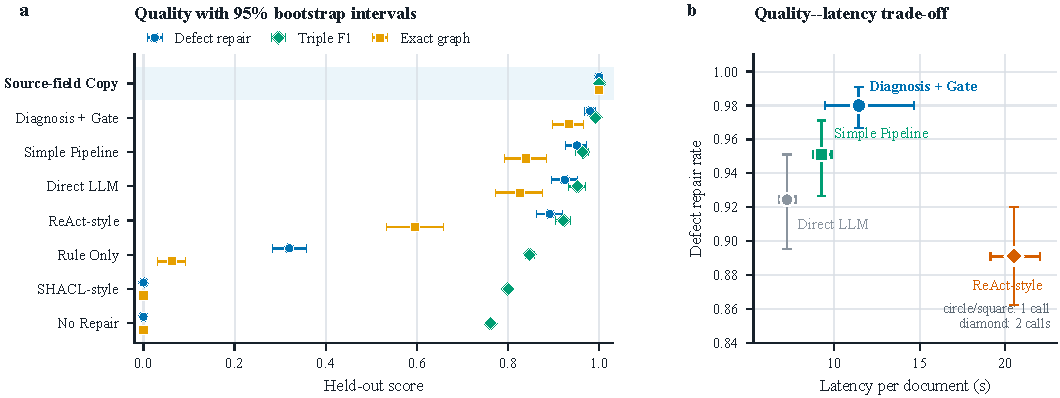
\includegraphics[width=0.98\textwidth]{figure/experiments/repair_benchmark_results.pdf}
\caption{Repair of added defects. \textbf{a}, Repair rate, triple F1, and exact match with 95\% CIs from document sampling. \textbf{b}, Scores and request times for methods using one or two calls.}
\label{fig:repair_benchmark_results}
\end{figure*}

\subsection{Repair of Model-Built Graphs}
\label{sec:eval:natural}

The input graphs have 87.99\% F1 and 65.78\% exact match
(Table~\ref{tab:natural_errors}). Diagnosis + Gate raises F1 to 92.48\%.
It reduces reference differences by 27.75\% and keeps all input triples
that match the reference. Simple has a mean difference reduction of
$-59.15\%$ on the 77 inputs with differences. It adds more differences
than it removes.

Diagnosis + Gate leads Simple by 4.40 F1 points (95\% CI: 3.07--5.77).
It leaves 1.03 fewer differences per document on average
(95\% CI: 0.77--1.32; Wilcoxon $p=3.18\times10^{-12}$).
Three graphs match exactly under Diagnosis + Gate and differ under Simple.
Zero show the reverse ($p=0.25$). Source-field Copy matches all references.

\begin{table*}[t]
\centering
\caption{Repair of model-built graphs. Difference reduction uses the 77 inputs that differ from the reference. Other scores use all 225 documents.}
\label{tab:natural_errors}
\small
\resizebox{\textwidth}{!}{%
\begin{tabular}{l c c c c c c c}
\toprule
Method & Parse & Non-exact inputs & Difference reduction & Facts kept & Over-repair & Triple F1 & Exact match \\
\midrule
Source-field Copy & 1.0000 & 77 & 1.0000 & 1.0000 & 0.0000 & 1.0000 & 1.0000 \\
Extracted graph, no repair & 0.9556 & 77 & 0.0000 & 1.0000 & 0.0000 & 0.8799 & 0.6578 \\
Simple Pipeline & 1.0000 & 77 & $-0.5915$ & 0.9971 & 0.2389 & 0.8807 & 0.6711 \\
Diagnosis + Gate & 0.9956 & 77 & 0.2775 & 1.0000 & 0.0292 & 0.9248 & 0.6844 \\
\bottomrule
\end{tabular}%
}
\end{table*}

\paragraph{Valid and invalid JSON inputs.}
The 215 valid JSON inputs have 92.09\% F1. Diagnosis + Gate reaches 93.53\%
and Simple reaches 88.85\% on these inputs. Among the 67 valid inputs with
reference differences, Diagnosis + Gate reduces the differences by 24.00\%
and raises F1 from 74.61\% to 79.22\%.
It keeps all 148 initially exact graphs exact.
The ten invalid inputs reach 69.91\% F1 after repair; zero match exactly.

\begin{figure}[t]
\centering
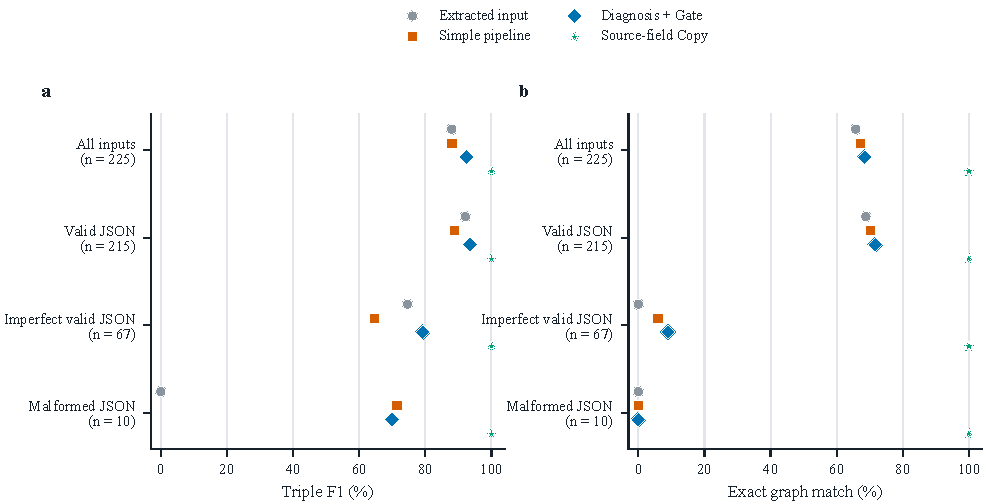
\includegraphics[width=0.98\textwidth]{figure/experiments/natural_stratified.pdf}
\caption{Repair scores by input type. The valid-JSON group shows repair of parsed graphs. The invalid-JSON group shows recovery from empty inputs.}
\label{fig:natural_stratified}
\end{figure}

\subsection{Prompt, Filter, and Edit-Selector Tests}
\label{sec:eval:router}
\label{sec:eval:mechanisms}

We test prompt text, filtering, and edit selection in turn.
On the saved Claude responses, filtering raises F1 from 98.95\% to 99.17\%
and reduces over-repair by 0.60 points. Repair stays at 98.00\% and exact
match at 93.33\%. The filter removes eight triples. All eight fail the
source check and differ from the reference.
Appendix~\ref{sec:eval:ablation} gives the full method table.

% Begin merged sections/audit_primary.tex
% Generated by exps/paper1_mechanism_audit/write_paper_tables.py
\begin{table*}[t]
\centering
\caption{Gemma prompt tests on 60 documents per input group. Each raw/gated pair uses the same response.}
\label{tab:matched_mechanisms}
\small
\resizebox{\textwidth}{!}{%
\begin{tabular}{llrrrr}
\toprule
Context & Output & Ctrl. repair & Ctrl. F1 & Natural F1 & Natural exact \\
\midrule
Base & Raw & 0.9750 & 0.9951 & 0.9185 & 0.6667 \\
Base & Gate & 0.9750 & 0.9962 & 0.9252 & 0.6667 \\
Diagnostic & Raw & 0.9250 & 0.9850 & 0.9079 & 0.6667 \\
Diagnostic & Gate & 0.9250 & 0.9861 & 0.9147 & 0.6667 \\
SHACL context & Raw & 0.9500 & 0.9912 & 0.9322 & 0.7000 \\
SHACL context & Gate & 0.9500 & 0.9912 & 0.9364 & 0.7000 \\
\bottomrule
\end{tabular}%
}
\end{table*}
% End merged sections/audit_primary.tex


The Gemma test uses 60 documents, 20 per source, with added-defect and
model-built inputs. Three prompts share the same instructions, cleanup,
temperature, and output limit. Each response is scored before and after
the same gate. Table~\ref{tab:matched_mechanisms} gives all six settings.
Table~\ref{tab:matched_cost} gives input tokens and request times.
Section~\ref{sec:impl:shacl} gives the SHACL prompt.

With filtering, the base prompt reaches 99.62\% F1 and 97.50\% repair on
added-defect inputs. The error-report prompt reaches 98.61\% F1 and 92.50\%
repair. The paired F1 change is $-1.01$ points
(95\% CI: $[-1.67,-0.38]$; $p=0.0082$).
On model-built inputs, Base + Gate reaches 92.52\% F1,
Diagnosis + Gate reaches 91.47\%, and SHACL Context + Gate reaches 93.64\%.
The Diagnosis--SHACL F1 difference is $-2.16$ points
(95\% CI: $[-5.26,0.02]$; $p=0.105$).

On model-built inputs with an error-report prompt, filtering raises F1 from
90.79\% to 91.47\%. The gain is 0.69 points
(95\% CI: 0.20--1.29; $p=0.0335$), with the same exact-match score.
Across the 360 responses, the gate rejects 27 triples.
All 27 differ from the reference.

\begin{figure}[t]
\centering
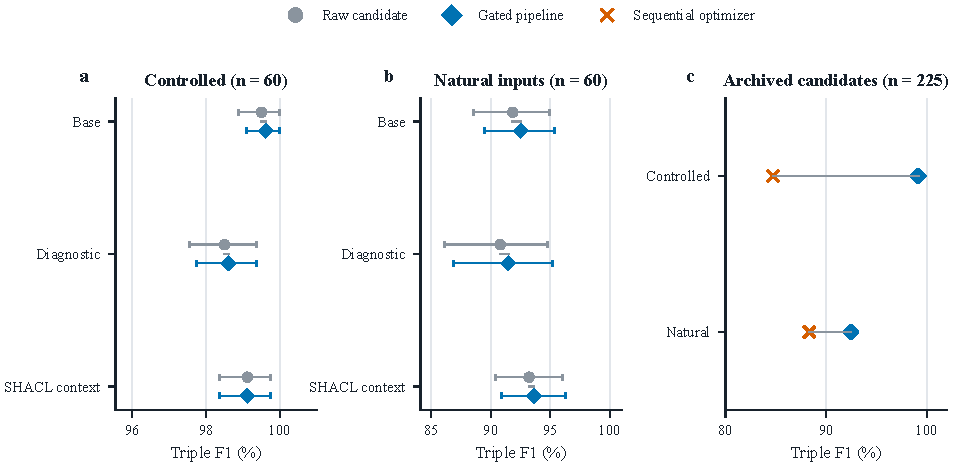
\includegraphics[width=0.98\textwidth]{figure/experiments/matched_mechanisms.pdf}
\caption{Prompt, filter, and selector tests. Panels a--b use Gemma outputs on 60 documents. Each raw/gated pair uses the same response. Bars show 95\% document-bootstrap CIs. Panel c uses saved Claude proposals for 225 documents.}
\label{fig:matched_mechanisms}
\end{figure}

% Begin merged sections/factorial_controls.tex
\paragraph{Testing cleanup, error reports, and filtering together.}
\label{sec:eval:factorial}

We switch input cleanup ($P$) and the error report ($D$) on or off.
The four prompt settings use 60 added-defect and 60 model-built inputs,
giving 480 Gemma responses. Each response is scored with and without the
gate ($G$). Each main effect averages over the other two switches.

\begin{table}[t]

\centering

\caption{Mean F1 changes in percentage points. Each input group has 60 paired documents. Each effect averages over the other two switches. CIs are 95\% document-bootstrap intervals. $p_H$ corrects the six main-effect tests with Holm correction.}
\label{tab:recovery_factorial}

\small

\begin{tabular}{llrrr}

\toprule

Input & Component & Change & 95\% interval & $p_H$ \\

\midrule

Controlled & Preprocessing & -0.028 & [-0.797, 0.778] & 1.000 \\

Controlled & Diagnosis & -0.651 & [-1.348, -0.056] & 0.164 \\

Controlled & Gate & +0.164 & [0.054, 0.301] & 0.156 \\

Natural & Preprocessing & +0.697 & [0.000, 1.905] & 1.000 \\

Natural & Diagnosis & -0.535 & [-2.376, 0.842] & 1.000 \\

Natural & Gate & +0.707 & [0.225, 1.316] & 0.086 \\

\bottomrule

\end{tabular}

\end{table}

All six Holm-corrected $p$ values exceed 0.05
(Table~\ref{tab:recovery_factorial}). The error report lowers mean F1
in both input groups. The gate raises mean F1 by 0.164 points on
added-defect inputs and 0.707 points on model-built inputs.
Across all input groups, the full filter rejects 47 triples:
17 have wrong document IDs and 30 fail source matching.
All 47 differ from the reference. The released scores also list the joint
switch effects and removals by each check.
% End merged sections/factorial_controls.tex


\paragraph{Tests of each filter check.}
We score 540 saved responses under eight filter settings, giving 4,320
outputs. The full filter rejects 28 triples: 11 have wrong document IDs
and 17 fail source matching. All 28 differ from the reference.
The other checks remove zero extra candidates in this sample.
All 21 adjusted check-comparison $p$ values exceed 0.05.
Appendix~\ref{sec:eval:individual_ablation} gives the table.

\paragraph{Edit selection.}
On the saved Claude proposals, the default selector with learned or equal
weights accepts zero edits on added-defect inputs. Repair stays at 32.00\%
and F1 at 84.72\%, the cleaned-input scores.
In the v2 runs, model-built inputs reach 88.33\% F1 with equal weights
and 87.99\% with learned weights. The learned trigger also reaches 87.99\%.
Removing edit cost raises added-defect F1 to 89.30\%.
Model-built F1 is 88.13\% in that setting.
The logs show missing fields in graphs with high profile scores.
Some useful additions receive scores of zero or less and are rejected.
Appendix~\ref{sec:eval:individual_ablation} gives all 13 settings, two prior
score forms, and 11,700 outcomes. Appendix~\ref{app:historical_diagnostics}
also gives earlier selector results and the call-policy test.

\subsection{Tests with Two Models}
\label{sec:eval:crossmodel}

We compare Direct LLM, Simple, and Diagnosis + Gate on 60 added-defect
inputs, 20 per source. The models are Claude Haiku and
\texttt{google/gemma-4-26B-A4B-it} \citep{ref_gemma4}.
Each method uses the same inputs, prompt form, temperature, and one-call
limit across models. Diagnosis + Gate has the highest repair rate with
both models (Table~\ref{tab:cross_model}). Its F1 lead over Simple is larger
with Claude. Gemma's direct outputs have higher F1 than Claude's.

\begin{table}[t]
\centering
\caption{Two-model results on the same 60 added-defect inputs.}
\label{tab:cross_model}
\small
\begin{tabular}{l l c c c}
\toprule
Model & Method & Repair & F1 & Exact \\
\midrule
Claude & Direct & 0.958 & 0.970 & 0.867 \\
Claude & Simple & 0.958 & 0.966 & 0.833 \\
Claude & \textbf{Diag.+Gate} & \textbf{0.975} & \textbf{0.991} & \textbf{0.917} \\
\midrule
Gemma & Direct & 0.958 & 0.988 & 0.883 \\
Gemma & Simple & 0.967 & 0.984 & 0.867 \\
Gemma & \textbf{Diag.+Gate} & \textbf{0.983} & \textbf{0.990} & \textbf{0.917} \\
\bottomrule
\end{tabular}
\end{table}

% Begin merged sections/receipt_followup.tex
\subsection{Source-Line Hints on New Receipts}
\label{sec:eval:receipt_followup}

In the first 60-receipt test, base and error-report prompts keep all input
graphs unchanged. Filtering lowers F1 from 79.44\% to 79.15\%.
It rejects an address because its spaces differ from the source.
Of 49 reference differences, 27 involve case, spaces, punctuation, or amount
format (Appendix~\ref{sec:eval:external_receipts}). We use these findings to
add field meanings, source-line hints, and a shared whitespace rule.

We set the index design on 20 new receipts, then fix it before testing 60
further receipts (Section~\ref{sec:framework:field_evidence}).
The first 60, development 20, and new test 60 receipts have different IDs
and different text after whitespace cleanup. Sampling uses seed 20260923.
Test labels are downloaded after all predictions are saved.
Every method receives the same field meanings, numbered source lines,
input graph, and instructions. Simple uses them directly.
Evidence Index adds field-line hints. SHACL adds rule-check context.
All three use the same whitespace rule in the filter.

Development F1 is 80.00\% for the input, 82.50\% for Simple,
85.00\% for Evidence Index, and 80.00\% for SHACL.
We keep one index design and all three methods for the test.
The main comparison is Evidence Index minus Simple in mean document F1.
The code and scoring rules are fixed before testing.

\begin{table*}[t]
\centering
\caption{Repair on 60 new receipts. Methods share field meanings, source lines, and the same whitespace check. Exact match uses the labelled fields.}
\label{tab:receipt_followup}
\small
\begin{tabular}{lrrrr}
\toprule
Method & Triple F1 & Exact graph & Normalized F1 & Facts kept \\
\midrule
Extracted input & 0.7833 & 0.3500 & 0.7958 & 1.0000 \\
Simple, raw & 0.7875 & 0.2833 & 0.8083 & 0.9250 \\
Simple, gate & 0.7875 & 0.2833 & 0.8083 & 0.9250 \\
Evidence Index, raw & 0.8333 & 0.4000 & 0.8625 & 0.9306 \\
Evidence Index, gate & 0.8351 & 0.4000 & 0.8643 & 0.9306 \\
SHACL context, raw & 0.7833 & 0.2833 & 0.8042 & 0.9347 \\
SHACL context, gate & 0.7833 & 0.2833 & 0.8042 & 0.9347 \\
\bottomrule
\end{tabular}
\end{table*}

On the new test, input F1 is 78.33\%. Simple, Evidence Index, and SHACL
reach 78.75\%, 83.51\%, and 78.33\% after filtering.
Simple gains $0.42$ points over the input (95\% CI: $[-4.17,5.00]$).
Evidence Index leads Simple by $4.76$ points
(95\% CI: $[2.50,7.26]$; paired randomization $p=0.0004$).
Exact match is 28.33\%, 40.00\%, and 28.33\% for the three methods.

The input has 52 fields that differ from the reference.
Simple recovers 16 of them and loses 15 exact input matches.
Evidence Index recovers 26 and loses 14. SHACL recovers 13 and loses 13.
The index fixes 11 punctuation differences and 6 text-boundary differences.
Among its 14 lost exact matches, 10 keep the same numeric amount and change
the display format.

A numeric check removes currency prefixes and thousands separators from
the total field. It gives 58/60 correct amounts for the input,
59/60 for Simple, 59/60 for Evidence Index, and 58/60 for SHACL.
After case and whitespace cleanup, F1 is 86.43\% for Evidence Index
and 80.83\% for Simple. The index improves both exact and cleaned-text scores.

The filter rejects 1 candidate. It differs from the reference and joins
address parts into text absent from the source. The count of rejected
reference matches is 0. Filtering raises indexed F1 by 0.18 points.
The other two methods keep the same F1.

Simple, Evidence Index, and SHACL change 31, 39, and 28 input graphs.
Their mean repair request times are 7.91, 7.88, and 8.11 seconds.
Mean input lengths are 1784, 2153, and 3404 tokens.
The 240 requests produce 60 extraction and 180 repair outputs.
Request times include pacing and retries. Each raw/gated score pair uses
one response.

\begin{figure}[t]
\centering
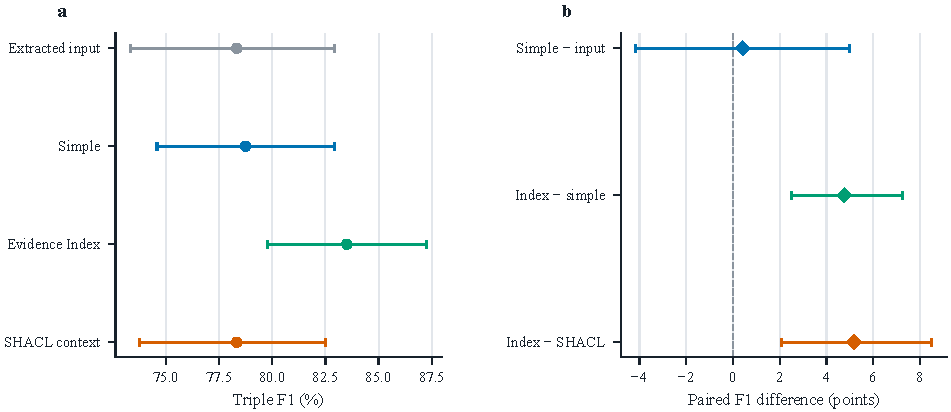
\includegraphics[width=0.98\textwidth]{figure/experiments/receipt_followup.pdf}
\caption{New receipt test. Left: mean F1 with 95\% document-bootstrap CIs. Right: paired F1 changes. All methods share field meanings and source lines.}
\label{fig:receipt_followup}
\end{figure}
% End merged sections/receipt_followup.tex

% Begin merged sections/receipt_context_controls.tex
\subsection{Comparing Source-Line Hints}
\label{sec:eval:recovery_ablation}

We compare six prompt settings on the same 60 new-test receipts.
The test uses 360 new Gemma responses from the same batch as the component
tests. All responses parse. Each setting keeps the full source and shares
the model, output limit, and filter.
The random index has about the same character length as the full index.

\begin{table}[t]

\centering

\caption{Source-line tests on 60 receipts. Each row uses the same model, source, output limit, and filter. Random hints have about the same character length as the index.}
\label{tab:recovery_index}

\small

\begin{tabular}{lrr}

\toprule

Context & Exact F1 & Normalized F1 \\

\midrule

Simple & 0.7917 & 0.8125 \\

Full index & 0.8351 & 0.8643 \\

Anchors only & 0.8351 & 0.8643 \\

Random index & 0.8167 & 0.8458 \\

Simple, no definitions & 0.8083 & 0.8292 \\

Full index, no definitions & 0.7470 & 0.7762 \\

\bottomrule

\end{tabular}

\end{table}

The full index leads Simple by 4.35 F1 points (95\% CI: 1.25 to 7.86).
Its Holm-corrected value is $p_H=0.065$ across five planned comparisons.
The full index and anchor lines alone have the same mean F1.
The full--random difference is 1.85 points
(CI: $[-0.65,4.52]$; $p_H=0.696$).
Removing field meanings from the full index lowers F1 by 8.81 points
(CI: $[4.23,13.39]$; $p_H=0.006$).
The Simple setting scores higher with field meanings removed in this batch.
These results show that field meanings help the indexed prompt choose values.

\begin{figure}[t]

\centering

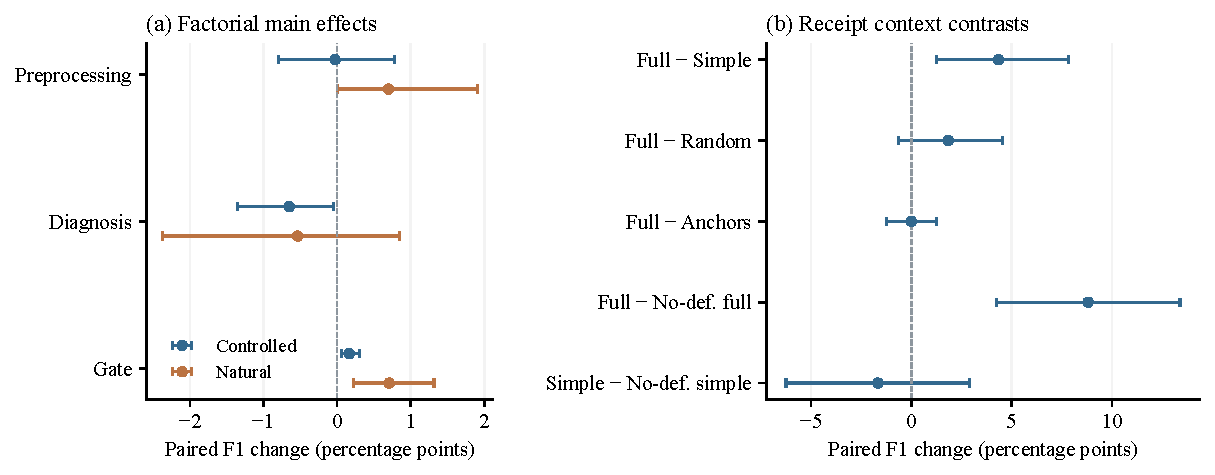
\includegraphics[width=0.98\textwidth]{figure/experiments/recovery_ablation.pdf}

\caption{Component and source-line tests. Points show mean paired F1 changes. Bars show 95\% CIs for each change. The component and receipt tests use separate Holm groups.}
\label{fig:recovery_ablation}

\end{figure}
% End merged sections/receipt_context_controls.tex

% Begin merged sections/reextraction_recovery.tex
\subsection{Repair versus Fresh Extraction}
\label{sec:eval:reextraction}

We reuse the 60 new-test receipts for four settings: repair or fresh
extraction, with or without the index. All settings share source lines,
field meanings, the document ID, and the output limit.
Repair also receives the existing graph. All 240 responses put JSON
inside Markdown fences. The fixed strict parser scores them as failures.

We then rescore the same responses after removing the fences and assigning
the known document ID to every output. This extra analysis gives 83.93\% F1
for indexed repair and 74.86\% for indexed fresh extraction.
The paired difference is 9.07 points (95\% CI: 5.22 to 13.10).
The repair calls use an existing graph; its creation cost is counted apart.
Appendix~\ref{app:reextraction_diagnostics} gives the strict scores,
fence-cleanup scores, ID errors, and source-line coverage.
The contract test fixes fence handling and ID assignment before collection.
% End merged sections/reextraction_recovery.tex

% Begin merged sections/cuad_contracts.tex
\subsection{Contract Field Test}
\label{sec:eval:cuad}

We use CUAD~\citep{ref_cuad} to test five fields: document name, agreement
date, effective date, expiration date or initial term, and governing law.
We select contracts with at most one distinct reference value per field
after whitespace cleanup and at most 40,000 source characters.
We keep the full source and check the positions of the labelled values.
Twenty official-training contracts form the development set.
All 56 official-test contracts that meet the rules form the test set.

We compare initial extraction, Simple repair, indexed repair, and indexed
fresh extraction. Both repair methods receive the same initial graph.
The indexed methods add field-line windows to the full source.
All settings share the Gemma model, field meanings, and a 4,000-token output
limit. Before collection, we set the code to handle JSON fences and assign
document IDs. We keep the prompts and selection rules fixed after one
development round.

\begin{table}[t]
\centering
\caption{Contract results on 56 documents. F1 checks exact text after whitespace cleanup. Lost counts correct input facts removed. The input row gives the initial graph cost; repair rows give the repair-call cost.}
\label{tab:cuad}
\small
\begin{tabular}{lrrrr}
\toprule
Output & F1 (\%) & Lost & New incorrect & Requests \\
\midrule
Initial extraction & 46.76 & 0 & 0 & 59 \\
Simple repair & 43.35 & 7 & 2 & 71 \\
Indexed repair & 44.84 & 5 & 12 & 69 \\
Indexed re-extraction & 44.12 & 8 & 32 & 71 \\
\bottomrule
\end{tabular}
\end{table}

Indexed repair reaches 44.84\% F1, compared with 46.76\% for the input,
a 1.92-point drop. It removes five correct input facts and adds twelve
facts that differ from the reference. Simple repair also scores below
the input.

Indexed repair leads indexed fresh extraction by 0.72 F1 points
(95\% paired CI: [-4.80,6.48]; sign-flip $p=0.810$).
The test gives 224 outputs from 270 requests, including retries.
Failed outputs are scored as empty graphs.
The score checks copied text against CUAD labels after whitespace cleanup.

\begin{figure}[t]
\centering
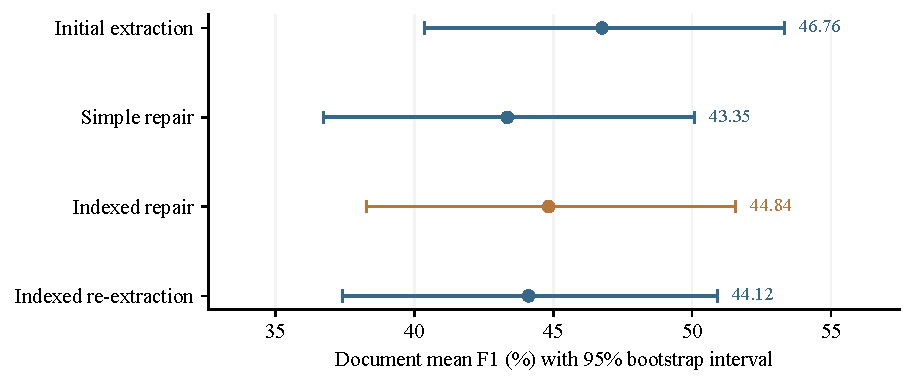
\includegraphics[width=0.88\textwidth]{figure/experiments/cuad_contracts.pdf}
\caption{Contract scores. Points show mean document F1. Bars show 95\% CIs for each method. The text gives the paired repair--extraction CI.}
\label{fig:cuad}
\end{figure}
% End merged sections/cuad_contracts.tex


\subsection{Human Review of Errors and Edits}
\label{sec:eval:human}

Task D checks 200 reference differences sampled from the 302 triple
differences in model-built inputs. Task E checks 200 actual edits sampled
from 598 edits across five settings. Both use random sampling with seed 42.
Each item is one difference or edit. A document can supply several items.
Reviewers see the source, schema, input graph, and named operation.
Task E also shows the full output graph. Method names and reference-quality
hints are hidden.

Two reviewers with computer-science backgrounds and Chinese reading skills
read the rules and practice examples. They then label the same 400 items
on their own. For each item, they answer two questions: is the input wrong
at this position (\texttt{is\_error}), and is the add or remove operation
acceptable (\texttt{repair\_acceptable})? They use 0, 1, or U and give reasons.
U means the shown evidence is too limited for a decision.
A third reviewer checks the source and graphs and resolves 154 items with
a disagreement by choosing between the two answers. The 246 agreed items
keep their labels. One edit-acceptance answer remains U.
We retain the original labels and agreement scores.

\begin{table}[t]
\centering
\caption{Human scores. Agreement and $\kappa$ use the two original 0/1/U answers. Positive counts use final labels. Acceptance rates use the cases with a 0 or 1 answer.}
\label{tab:human_review}
\small
\begin{tabular}{llrrrr}
\toprule
Task & Judgment & Agreement & $\kappa$ & Positive / certain & U \\
\midrule
D & Input error & 80.0\% & 0.600 & 95/200 (47.5\%) & 0 \\
D & Suggested edit acceptable & 62.0\% & 0.334 & 86/200 (43.0\%) & 0 \\
E & Input error & 86.0\% & 0.677 & 134/200 (67.0\%) & 0 \\
E & Actual edit acceptable & 65.0\% & 0.128 & 134/199 (67.3\%) & 1 \\
\bottomrule
\end{tabular}
\end{table}

Reviewers find input errors in 95/200 reference differences and accept
86/200 suggested edits. They accept 134/199 actual edits; one is uncertain.
A missing value can be correct, yet adding it can leave two values in a
field that allows one. The input-error and edit questions cover these
two decisions. Original edit agreement in task E is 65.0\% with
$\kappa=0.128$.

\begin{table}[t]
\centering
\caption{Actual-edit acceptance by setting. The random sample has different group sizes. Rates use edits with a clear decision.}
\label{tab:human_review_by_config}
\small
\begin{tabular}{lrrr}
\toprule
Configuration & Sampled & Acceptable & U \\
\midrule
Archived Simple & 105 & 63/104 (60.6\%) & 1 \\
Archived Diagnosis + Gate & 41 & 25/41 (61.0\%) & 0 \\
Gemma Base + Gate & 16 & 13/16 (81.3\%) & 0 \\
Gemma Diagnosis + Gate & 16 & 13/16 (81.3\%) & 0 \\
Gemma SHACL Context + Gate & 22 & 20/22 (90.9\%) & 0 \\
\bottomrule
\end{tabular}
\end{table}

The sample has 105 Archived Simple edits, 41 Archived Diagnosis + Gate
edits, 16 Gemma Base + Gate edits, 16 Gemma Diagnosis + Gate edits,
and 22 Gemma SHACL Context + Gate edits.
The table reports the share of accepted edits in each group.

\subsection{Discussion}
\label{sec:eval:failure}

Source format guides the choice of repair method.
A parser can copy fields from records that list names and values.
Receipts require choosing values from the full text. Source-line hints
raise F1 in the new receipt test. The later index tests show the role of
field meanings: removing them lowers indexed F1 by 8.81 points.
On contracts, indexed repair reaches 44.84\% F1, compared with 46.76\%
for the input. Keeping correct input fields is a clear target for repair.

The tests also show what the filter changes. Source and document-ID checks
remove extra triples. Field selection happens in model generation and in
the first-value rule. For example, a source can contain both a subtotal
and a final amount. The repair method must choose the right one for ``total''.
This calls for checks that use the meaning of the relation as well as the
presence of the value in the text.

Human reviewers accept 67.3\% of the sampled edits across five settings.
They find input errors in 47.5\% of the sampled reference differences.
The Archived Diagnosis + Gate sample has 25/41 accepted edits.
Together with the raw labels and reasons, these scores help locate errors
in field choice and individual edit decisions.

\subsection{Code and Data}

Code, prompts, data lists, model outputs, and scoring scripts are at
\url{https://github.com/turambar928/MCP_based_KG_construction}.
Each run saves model settings, parse status, requests, and token use.
All responses are kept. Experiment READMEs give data sources, samples,
checksums, and commands.

The human-review files include fixed task rules, the scorer, summary results,
original agreement scores, and sample lists. Individual answers and reasons
are kept private. Receipt scores use SROIE's human field labels.

\begin{table}[t]
\centering
\caption{Research questions and test results.}
\label{tab:research_answers}
\small
\begin{tabularx}{\textwidth}{@{}p{0.10\textwidth}XX@{}}
\toprule
Question & Comparison & Finding \\
\midrule
RQ1 & Added defects and model-built graphs
& Diagnosis + Gate improves repair and F1. Direct copying matches all Chinese record references. \\
RQ2 & Shared prompts and responses; source-line hints; edit selectors
& Source and ID checks remove extra triples. The receipt index raises F1. Error reports lower mean F1 in matched tests. Equal selector weights score above learned weights on model-built inputs. \\
RQ3 & Receipt and contract repair versus fresh extraction
& The receipt test favours the existing graph after fence and ID cleanup. Indexed contract repair scores below the initial graph. \\
\bottomrule
\end{tabularx}
\end{table}
